\documentclass{article}
\usepackage[utf8]{inputenc}
\usepackage[english]{babel}
\usepackage{multicol}
\usepackage{natbib}
\usepackage{graphicx}
\usepackage{float}
\usepackage{amsfonts}
\usepackage{amssymb}
\usepackage[bottom]{footmisc}
\usepackage{listings}
\usepackage{hyperref}
\usepackage{pifont}
\usepackage{tabularx}
\newcommand{\tick}{\ding{51}}
\newcommand{\cross}{\ding{54}}

\lstdefinestyle{codels}{
    basicstyle=\ttfamily\footnotesize,
    breakatwhitespace=false,         
    breaklines=true,                 
    captionpos=b,                    
    keepspaces=true,                 
    showspaces=false,                
    showstringspaces=false,
    showtabs=false,                  
    tabsize=3,
    frame=single, 
    label=main,
}

\lstset{style=codels}

\setlength{\parindent}{0em}
% \setlength{\parskip}{1em}

\begin{document}

\begin{titlepage}

    \center

    
\includegraphics[scale=0.5]{AzuGryphonSharp.png} %\vspace{0.5cm}

    \huge  \textbf{GryphonSharp v1}

    \vspace{2cm}

    \Large \textbf{Anton Sukachev, a.sukachev@lancaster.ac.uk}

    School of Computing and Communications

    Lancaster University

    \vfill

    Coordinator: Abe Karnik (a.karnik@lancaster.ac.uk)\endgraf
    Research group: Human Computer Interaction

\end{titlepage}
\pagebreak

\tableofcontents
\pagebreak
% \begin{multicols*}{2}
    

\begin{abstract}
    Write up abstract
\end{abstract}

\section{Introduction}
Since the first computers, there has existed a strong need for a high-level programming language that would allow users to quickly and efficiently code applications and systems that they need for their businesses, personal projects or even games.  

This research has a few distinctive objectives it attempts to address:
\begin{itemize}
    \item A set of questions in the section \nameref{sec:motive}.
    \item Proposes a design for creating simple programs through G\# language.
    \item Presents implementation of G\# VPE.
\end{itemize}

// Aims of this research




\section{Background}
Unfortunately, due to the scope of research and novelty of the topic, there is no way to easily pinpoint exact beginning of the programming in general. For this reason, the research will begin to explore programming since the appearance of first languages.

\subsection{First abstract language}
The first ever abstract language appeared around 1969-1973 and it rapidly replaced assembly language which offered ‘one-at-a-time’ instruction in a semi-readable for human format. The C Programming Language quickly became a legend among programmers, especially those working on a very first UNIX operating system\citep{ritche_clang}.
The C programming language introduced a wide range of abstract paradigms that programmers could utilize to swiftly develop readable programs where they can orient freely and extend to their needs. Some of the examples of such paradigms include: struct, enum and array indexing with the following syntax:

\begin{lstlisting}[caption=C array indexing]
variable[2]
other_variable[0]
\end{lstlisting}

Programs that would otherwise require hours of revision and coding could be written in a matter of minutes, if not seconds. After C language, a major abstract language at a time, was standardized by ANSI, it became the primary language for most computing systems.  

Despite being a standard for most, if not all, computing systems, the language was platform-specific, meaning different platforms would have specific implementations, hence compiled executables could only be run on the platforms for which executables were explicitly compiled. That way executables compiled for Windows would not run on MacOS/Linux Unix systems.

Unlike most, C language offers naked address referencing, meaning any given number could be converted into address in memory and backwards. This low level access to actual computer memory is strongly tied to memory leaks, critical security leaks, and even unwanted overflows that, if left unchecked, could violate kernel space from user space, which in turn could trigger kernel panic.\citep{6234805} Not only extremely low-level access that the C language provides poses severe vulnerability risk to the entire operating system, but it also requires significantly advanced memory management systems written by the applications' developers. In contrast, languages such as Java or C\# have built-in memory management that automatically frees memory when instances no longer accessible.
For these reasons C language simply did not offer enough abstraction, security, and flexibility to aid development of complex programs.\citep{schmidt_1977_some}

\subsection{First Visual Programming Environments}
Visual Programming Environments (henceforth VPE) was introduced for educational purposes first appearing in 2003 for Intel's Computer Clubhouses where young could learn computer technologies. Original designs of scratch were solely intended for young by adding visual programmable elements that manipulate media on screen.\citep{demrkiran_2021_an}
Scratch UI uses sturdy design principles that achieve it's ultimate goal i.e. Single Window with multiple tabs ensures there is always visible primary components such as scene or code.

\subsection{Minecraft and Redstone}
Minecraft is a computer game that was introduced in 2009. Minecraft opened a new genre - Sandbox. Sanbox genre, effectively, allowed players to manipulate their environaments and shape them visually how they see fit. Game introduced first few 'quests' that introduced player to the game, which then left player to explore world on their own. Minecraft is extremely successful, but not for a straightforward 'because of this and that' reasons. \citep{baek_2020_mining}
Why Minecraft game that has nothing to do with teaching and programming\citep{baek_2020_mining} (at the very least initially, it was designed for self-entertainment by creating stories using creative tools that the game provided\citep{booch_2013_from}) has a communities which focus heavily on implementing complex computing systems (even entire CPU architectures in Minecraft using nothing else but plain single-thread Redstone).\citep{matteson_2017_a}

\subsection{Transpilers, an upgrade to existing languages}
Transpilers take source code and compile into other source code. This is 'transpilation'.\citep{cifuentes_1998_assembly}

\subsection{Blockly and general-purpose VPE}
Blockly was a good take on general-purpose VPE. It uses transpiler principles to interpret visual representation of a code.\citep*{7369000} It support wide range of target languages, however, currently, without specifically designed environment, Blockly, out-of-the-box, only supports few paradigms: functions, variables, arithmetic operations, flow control (loops, if statements) and a few more basic primitives like lists and color.\footnote{https://developers.google.com/blockly}
Blockly, natively, is only a set of theories and findings that build on top of preexisting VPE 'Scratch'.\citep{8120404} Despite it having rich and extensible documentation, Blockly is just a set of tools for creating VPEs.\citep{whitley_2006_evidence,bresson_2007_musical}





\section{Motivation}
\label{sec:motive}
How C achieved it's purpose?
Why has it became so popular?

How C represented basic programming constructs (for, while loops, if statements)?
When and why it fails?

Why Scratch became so popular?
How Scratch aims to achieve their aims?

Scratch is limited by Scratch VM.

Transpilers are interesting take on simplifying development.
Any attempts to generate code from Visual Programming Environments - refer to Blockly.


// write up

\section{System Design}
Previously mentioned transpilers were 'the next step' towards higher languages that might provide task-specific abstraction level and paradigms for easy development of said tasks.\citep*{gribova_2013_ontology} For example, many game studios that started working in limited language such as Lua had to either rewrite their entire game on a different engine under different programming language. However, since introduction of transpilers that use higher-level or simpler languages to transpile to low-lever or complex languages, one of the most popular examples (in addition to mentioned Typescript-Javascript transpiler) being CSharp.lua\footnote{https://github.com/yanghuan/CSharp.lua} which takes c\# code and transpilers it into Lua code retaining most, if not all original language features such as reflection, polymorphism, encapsulation etc.

In this project, it was decided to utilize offline transpiler. This decision is motivated by strong presence of high-level heavily optimized languages such as Java, Javascript, C\#, Python, C++ and others. In contrast, the other choices were: Compiler and Interpreter.
Interpreter is an algorithm which uses calls and translates them one by one into bytecode, all of this 'interpretation' is happening at runtime and therefore creates huge overhead because every instruction the interpreter executes, essentially has to be looked up before it can be executed. Look up of interpreters is \textit{usually} capped at RAM latency, rather than CPU cache latency, meaning look up of instructions happens in RAM in worst case scenario.
Compiler both JIT and AOT require significant investment of time to design and implement from scratch. For purposes of this research, creating custom G\# to machine code compiler would be infeasible and would simply go outside of this project's scope.








\section{Language Design}
\label{sec:landes}
Design will be split into multiple sections, this is because over the duration of the project this has changed a lot and evolved over the duration of the research addressing one issue at a time, but starting from scratch every time.

\subsection{Starcraft II inspired Behaviour Oriented Design}
\citep*{d2857949266349429ebd6e5db6c1d3a3}
// write up
\subsection{Node-like Shader Editor Design}
\citep{kiper_1997_criteria, coronado_2020_visual}
// write up
\subsection{Unreal Engine Blueprints inspired Design}
// write up
\subsection{Stateless Node Editor}
\citep*{8120404}
// write up




\section{Implementation}
\subsection{Intermediate GryphonSharp Representation}
Intermediate G\# Representation (henceforth G\# IR) is a JSON-structured file containing code, data and metadata for both Transpiler and Node Editor.
Node Editor metadata: 
\begin{itemize}
    \item \lstinline[columns=fixed]{bgSizes} \newline
    This instructs Node Editor how zoomed in the code map currently is.
    \item \lstinline[columns=fixed]{stagePos} \newline
    This tells Node Editor the last position the code map.
    \item \lstinline[columns=fixed]{nodeCount} \newline
    This is used for node id-ing, in other words, this value is assigned to new nodes on creation then incremented by 1.
    \item \lstinline[columns=fixed]{dataCount} \newline
    This is the same as nodeCount but used for id-ing data, again, when data is first introduced, it will be assigned this value, then the value will be incremented by 1.
\end{itemize}
When this metadata is parsed into the Node Editor it will load 'preferences' from the last save of the document.
G\# IR also has transformer metadata, however, it is used for both Node Editor and transformer. This metadata defines the type that is being parsed out or in to the function. This is later used for transpiler-side validation in case the G\# source was modified by hand.

\subsection{Incomplete Components}
Following subsections will include incomplete or unfinished components of this project. Generally, just like in the proposal of the GryphonSharp, the 3 key components this research was trying to achieve were: Language Server (GryphonSharp-Overwatch), G\#-to-C\# Transpiler (GryphonSharp-Transpiler), Visual Node Editor (GryphonSharp-vscode). Every component is detailed and documented in the following subsections.

\subsubsection{Language Server}
Originally, Language Server, codenamed 'Overwatch', was planned to be implemented with VSCode language server protocol.\footnote{https://code.visualstudio.com/api/language-extensions/language-server-extension-guide}
The Overwatch language server handles multiple tasks listed below.
\begin{itemize}
    \item \textbf{Type-Safety Enforcer} \newline
    When user tries to connect nodes in the node editor, types of connectors are evaluated through Overwatch server request. Overwatch, being connected to Omnisharp server, will evaluate validity of type parsing and return boolean with TRUE value if parsing type is 'legal' for the connector, otherwise it will return FALSE, which will instruct node editor to highlight connection is 'illegal'. Highlight can either allow connection with red-error cross across illegal connection (can be seen in figure \ref{fig:badcon}) or prevent connection altogether and raise an error through message box (can be seen in figure \ref{fig:badconerror}).
    \begin{figure}[H]
        \centering
        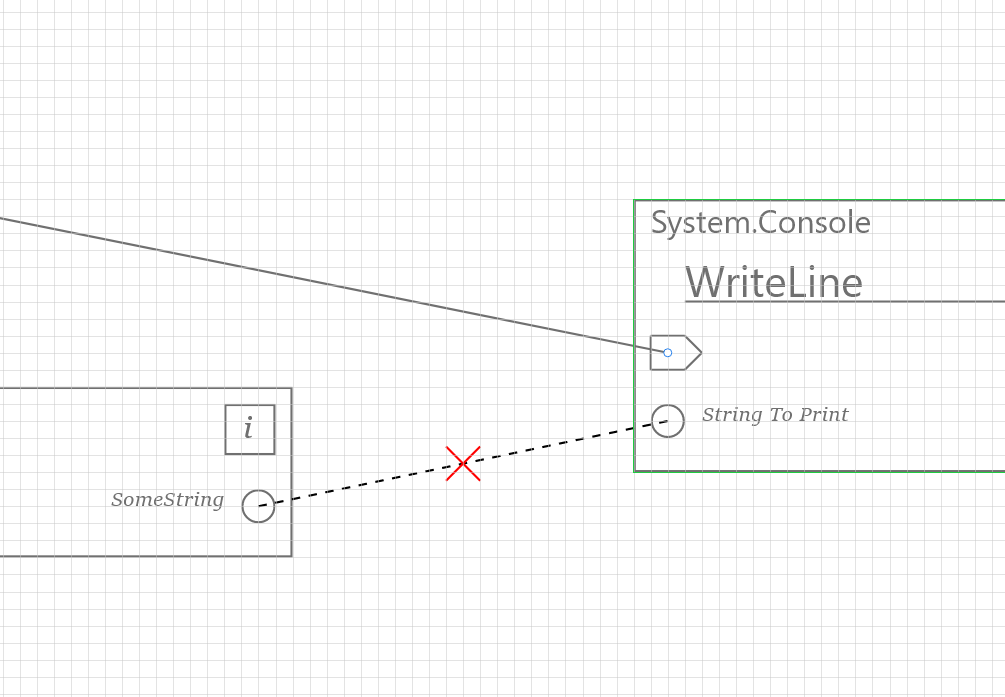
\includegraphics[width=1\textwidth]{Capture.PNG}
        \caption{Illegal Connection}
        \label{fig:badcon}
    \end{figure}
    \begin{figure}[H]
        \centering
        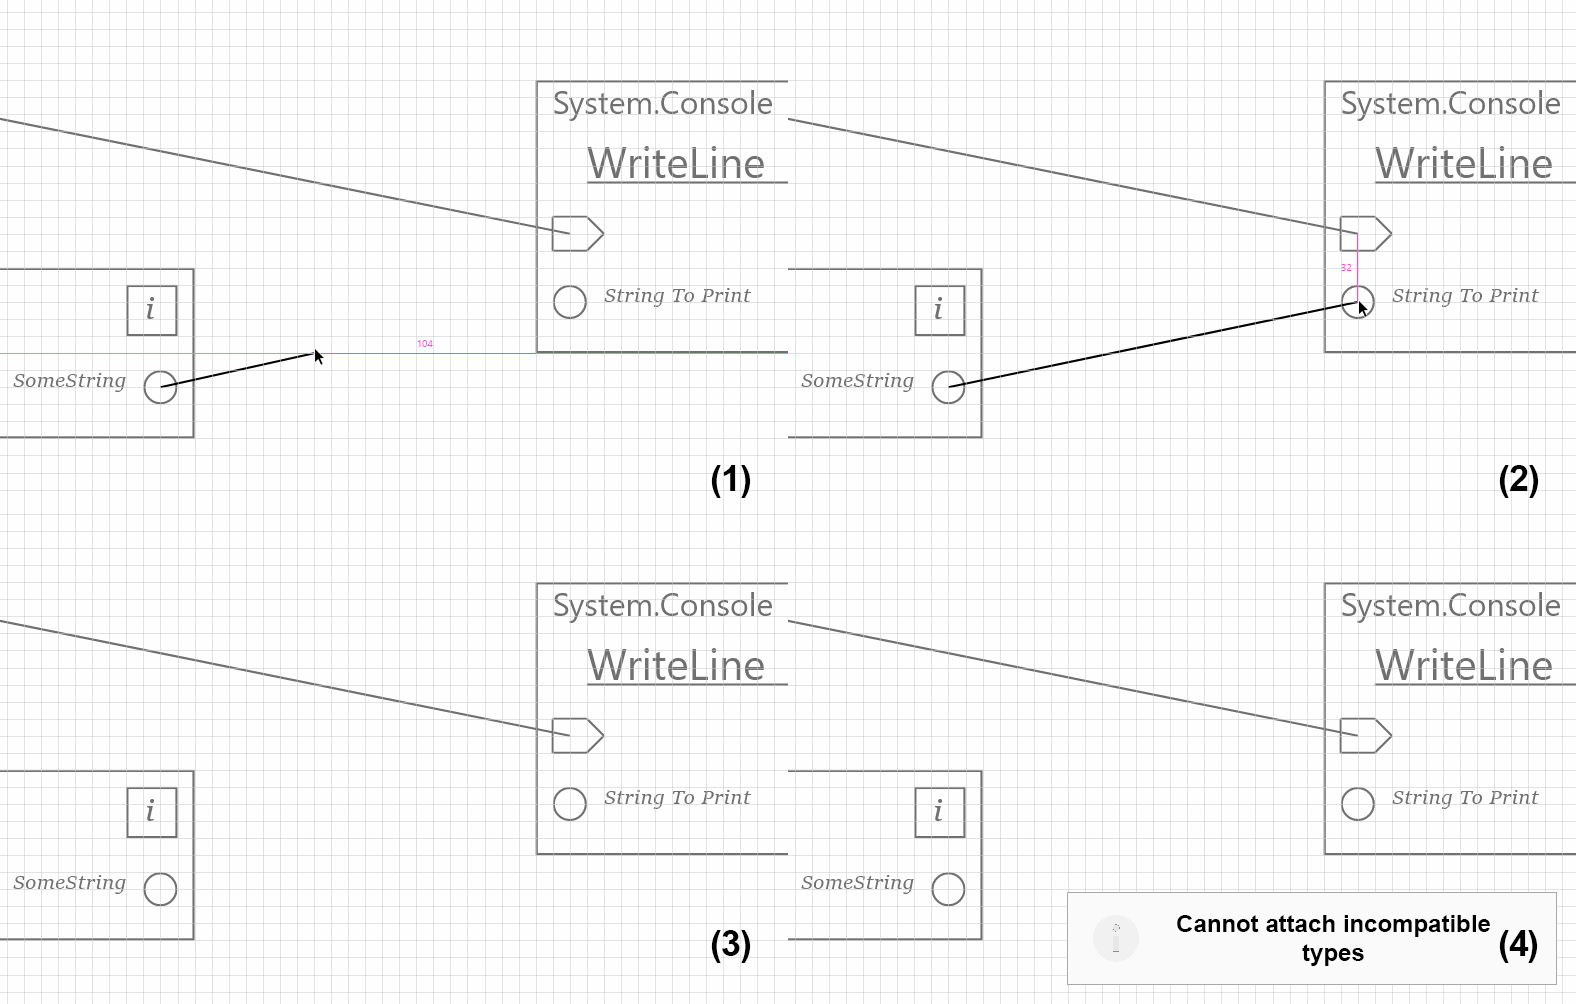
\includegraphics[width=1\textwidth]{illegalmove.png}
        \caption{Illegal Connection}
        \label{fig:badconerror}
    \end{figure}
    \item \textbf{Type Discovery} \newline
    When user attempts to parse a type into a empty space in the node editor, this will prompt user with function suggestions that match the parsed type.
    \item \textbf{Logic Evaluation} \newline
    When user constructs loops without exist clauses, such as while(true) loops or implement strange if statements, such as if(false), this will do a basic evaluation of the logic through existing tools in Omnisharp server.
    \item \textbf{Autocompletion} \newline
    When user types in a name of a function, variable, class or any other language construct, this will ask Omnisharp for Intellisense suggestions, which are then parsed into Node Editor for display.
    \item \textbf{Source Watcher} \newline
    When user makes changes to any of the files, Node Editor will notify VSCode of any workbench changes. These workbench changes are also parsed into language server. When the changes are made to source files or project files, language server will invoke G\#-to-C\# transpiler task.
\end{itemize}
\subsubsection{G\#-to-C\# Transpiler}
This is the actual transpiler that will convert G\# IR into C\# source code by the means of CodeDOM Microsoft package. CodeDOM allows construction of source code in readable format and supports all features of C\# language that are available to developers. CodeDOM is a powerful execution graph builder that supports C\# and IronPython transpilation. However, it can be defined, through a transformer factory, to translate into any other language according to the language's rules.
\subsubsection{Visual Node Editor}
Node Editor (in code is referred to as NE) is the primary focus of this research. Visual design of the editor is explained in-depth in section \nameref{sec:landes}. In this section, however, only the technical side of editor will be discussed.
Visual Node editor is an extension for a popular Electron app "Visual Studio Code"\footnote{https://code.visualstudio.com/}. Extension is written in typescript ES2015 and has 2 primary parts within the extension: Editor and Extension (sometimes referred to as simply frontend for Editor and backend for Extension). 

Frontend of NE is an html page covered by a Konva canvas. Konvajs canvas is a high-performance canvas for drawing nodes. It has powerful API and has some very promising demos, some of which are: fully functional Google-like spreadsheets, react-konvajs which is used by some of high-end applications such as Polotno.\footnote{https://polotno.dev/}
User can manipulate nodes in the editor which will be written into a \lstinline[columns=fixed]{*.gs} file upon saving. G\# (or \lstinline[columns=fixed]{*.gs}) files contain JSON intermediate representation (IR) of G\#. This JSON contains a lot of metadata for both NE and transpiler. Furthermore, JSON is plaintext serializable data structure, meaning it can be used seamlessly with code transformation tools, version control tools, and even modified by hand.
Frontend of NE is written in Typescript, unlike extension it has slightly different compilation and deployment pipelines. Frontend has to be compiled 'for browser', since, as stated above, VSCode is only a chromium that displays webpage, but has a backend that allows it to interact with operating system. Unfortunately, TypeScript doesn't support compilation for Browser runtime, which means the code will have to be bundled. This projects takes advantage of Rollup bundler, which compiles Typescript code into ES6, but the transforms it through iteration of dependency tree. Source files, along with any referenced NodeJS libraries, bundled into a single \lstinline[columns=fixed]{*.js} file that can be instantly executed by NE frontend.
The second part of the NE is backend. Backend is written in Typescript as well and can be natively run by NodeJS runtime. Due to limitation and old technology used in VSCode, backend code is still compiled into deprecated CommonJS code. Extension code is then injected into a developer instance of VSCode. For release versions, code is bundled and executed as a module when added.

\section{Discussion}
This project was heavily time-constrained and therefore was left in a work-in-progress state.






\section{Appendix}

% \begin{figure}[H]
%     \centering
%     \includegraphics[width=1\textwidth]{}
%     \caption{Gantt Chart}
%     \label{fig:gantt}
%     \end{figure}

% \end{multicols*}
\pagebreak
\bibliographystyle{plain}
\bibliography{refs.bib}
\end{document}
